%%%%%%%%%%%%%%%%%%%MAIN_OPTIONS%%%%%%%%%%%%%%%%%%%
\documentclass[a4paper, 14pt]{article}

%% Работа с русским языком
\usepackage{cmap}					% поиск в PDF
\usepackage{hyperref}				% гиперссылки
\usepackage[warn]{mathtext} 		% русские буквы в формулах
\usepackage[T2A]{fontenc}			% кодировка
\usepackage[utf8]{inputenc}			% кодировка исходного текста
\usepackage[english,russian]{babel}	% локализация и переносы

%% Дополнительная работа с математикой
\usepackage{amsfonts,amssymb,amsthm,mathtools} % AMS
\usepackage{amsmath}
\usepackage{icomma} % "Умная" запятая: $0,2$ --- число, $0, 2$ --- перечисление

%% Номера формул
%\mathtoolsset{showonlyrefs=true} % Показывать номера только у тех формул, на которые есть \eqref{} в тексте.

%%FONTS_Packadges
\usepackage{euscript} % Шрифт Евклид
\usepackage{mathrsfs} % Красивый матшрифт

%% Свои команды
\DeclareMathOperator{\sgn}{\mathop{sgn}}

%% Перенос знаков в формулах (по Львовскому)
\newcommand*{\hm}[1]{#1\nobreak\discretionary{}
	{\hbox{$\mathsurround=0pt #1$}}{}}

%%% Работа с картинками
\usepackage{graphicx}  % Для вставки рисунков
\graphicspath{{pictures/}{images2/}}  % папки с картинками
\setlength\fboxsep{3pt} % Отступ рамки \fbox{} от рисунка
\setlength\fboxrule{1pt} % Толщина линий рамки \fbox{}
\usepackage{wrapfig} % Обтекание рисунков и таблиц текстом
\usepackage[section]{placeins}
\usepackage{subcaption}

%% Работа с таблицами
\usepackage{array,tabularx,tabulary,booktabs} % Дополнительная работа с таблицами
\usepackage{longtable}  % Длинные таблицы
\usepackage{multirow} % Слияние строк в таблице

%%Links
\hypersetup{
	colorlinks=true,
	linkcolor=black,
	filecolor=magenta,      
	urlcolor=blue,
}

%%% Программирование
\usepackage{etoolbox} % логические операторы

%%% Страница
\usepackage{extsizes} % Возможность сделать 14-й шрифт
\usepackage{geometry} % Простой способ задавать поля
\geometry{top=25mm}
\geometry{bottom=35mm}
\geometry{left=20mm}
\geometry{right=20mm}
\usepackage{indentfirst}
%
\usepackage{fancyhdr} % Колонтитулы
\pagestyle{fancy}
\renewcommand{\headrulewidth}{0mm}  % Толщина линейки, отчеркивающей верхний колонтитул
%\lfoot{Нижний левый}
%\rfoot{Нижний правый}
%\rhead{Верхний правый}
%\chead{Верхний в центре}
%\lhead{Верхний левый}
% \cfoot{Нижний в центре} % По умолчанию здесь номер страницы

\usepackage{setspace} % Интерлиньяж
%\onehalfspacing % Интерлиньяж 1.5
%\doublespacing % Интерлиньяж 2
%\singlespacing % Интерлиньяж 1

\usepackage{multicol,caption}

\newenvironment{Figure}
{\par\medskip\noindent\minipage{\linewidth}}
{\endminipage\par\medskip}

\usepackage{enumitem}
\usepackage{amssymb}
\usepackage{xcolor}
%%% Зачеркнутый текст
\usepackage[normalem]{ulem}


\author{Каграманян Давид}
\title{Обзор статитьи}
\date{\today}

\begin{document}
	\thispagestyle{empty}
	\begin{center}
		\textit{Федеральное государственное автономное учреждение \\
			высшего профессионального образования}
		\vspace{0.5ex}
		
		\textbf{НАЦИОНАЛЬНЫЙ ИССЛЕДОВАТЕЛЬСКИЙ УНИВЕРСИТЕТ \\ <<ВЫСШАЯ ШКОЛА ЭКОНОМИКИ>>}
		
		Московский институт электроники и математики им. А.Н. Тихонова
	\end{center}
	\vspace{13ex}
	
	\begin{center}
		\vspace{13ex}
		\textbf{П\,Р\,А\,К\,Т\,И\,Ч\,Е\,С\,К\,А\,Я\,  \,Р\,А\,Б\,О\,Т\,А}
		\vspace{1ex}
		
		Обзор статьи\\

		\textbf{\textit{<<Mathematical Description of the Microstructural Modific>>}}
		\vfill
		
		\begin{flushright}
			\noindent
			\textit{Каграманян Давид Геворгович}

			\textit{студент информатики и вычислительной техники \\(группа БИВ184.1)}
			
		\end{flushright}
		Москва \the\year{}
	\end{center}
	
	\newpage
	\tableofcontents
	\newpage
	\section{Введение}
	
	Микроструктура металлов может состоять из аустенита, феррита, баинита и мартензита. В процессе термической и физческой обработки изменяются механические качества сплава. Они зависят от:
	 \begin{itemize}
	 
		\item состава сплава
		
		\item параметров обработки
		
		\item микроструктуры до обработки

	\end{itemize}

	Перлит - эвтектоидная смесь двух фаз: феррита и цементита
	
	Феррит - фазовая составляющая сплавов железа
	
	Цементит - карбид железа $F_3 C$
	
	Аустенит -  высокотемпературная гранецентрированная модификация железа и его сплавов
	
	 
	\section{Теория}

	Сфероидизацией перлита называют процесс превращения перлитной составляющей в сфероидальные выделения цементита.
	Пластинчатый перлит превращается в зернистый, в результате чего значительно уменьшаются твёрдость и прочность, но повышается пластичность металла.

	
	\begin{figure}[h!]
		\centering
		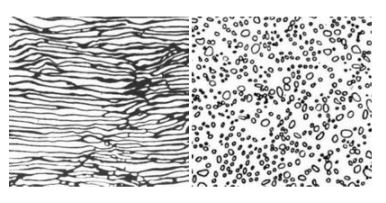
\includegraphics[scale=0.8]{images/пластзерн}
		\caption{пластинчатый и зернистый перлит}
	\end{figure}
	
	\begin{figure}[h!]
		\centering
		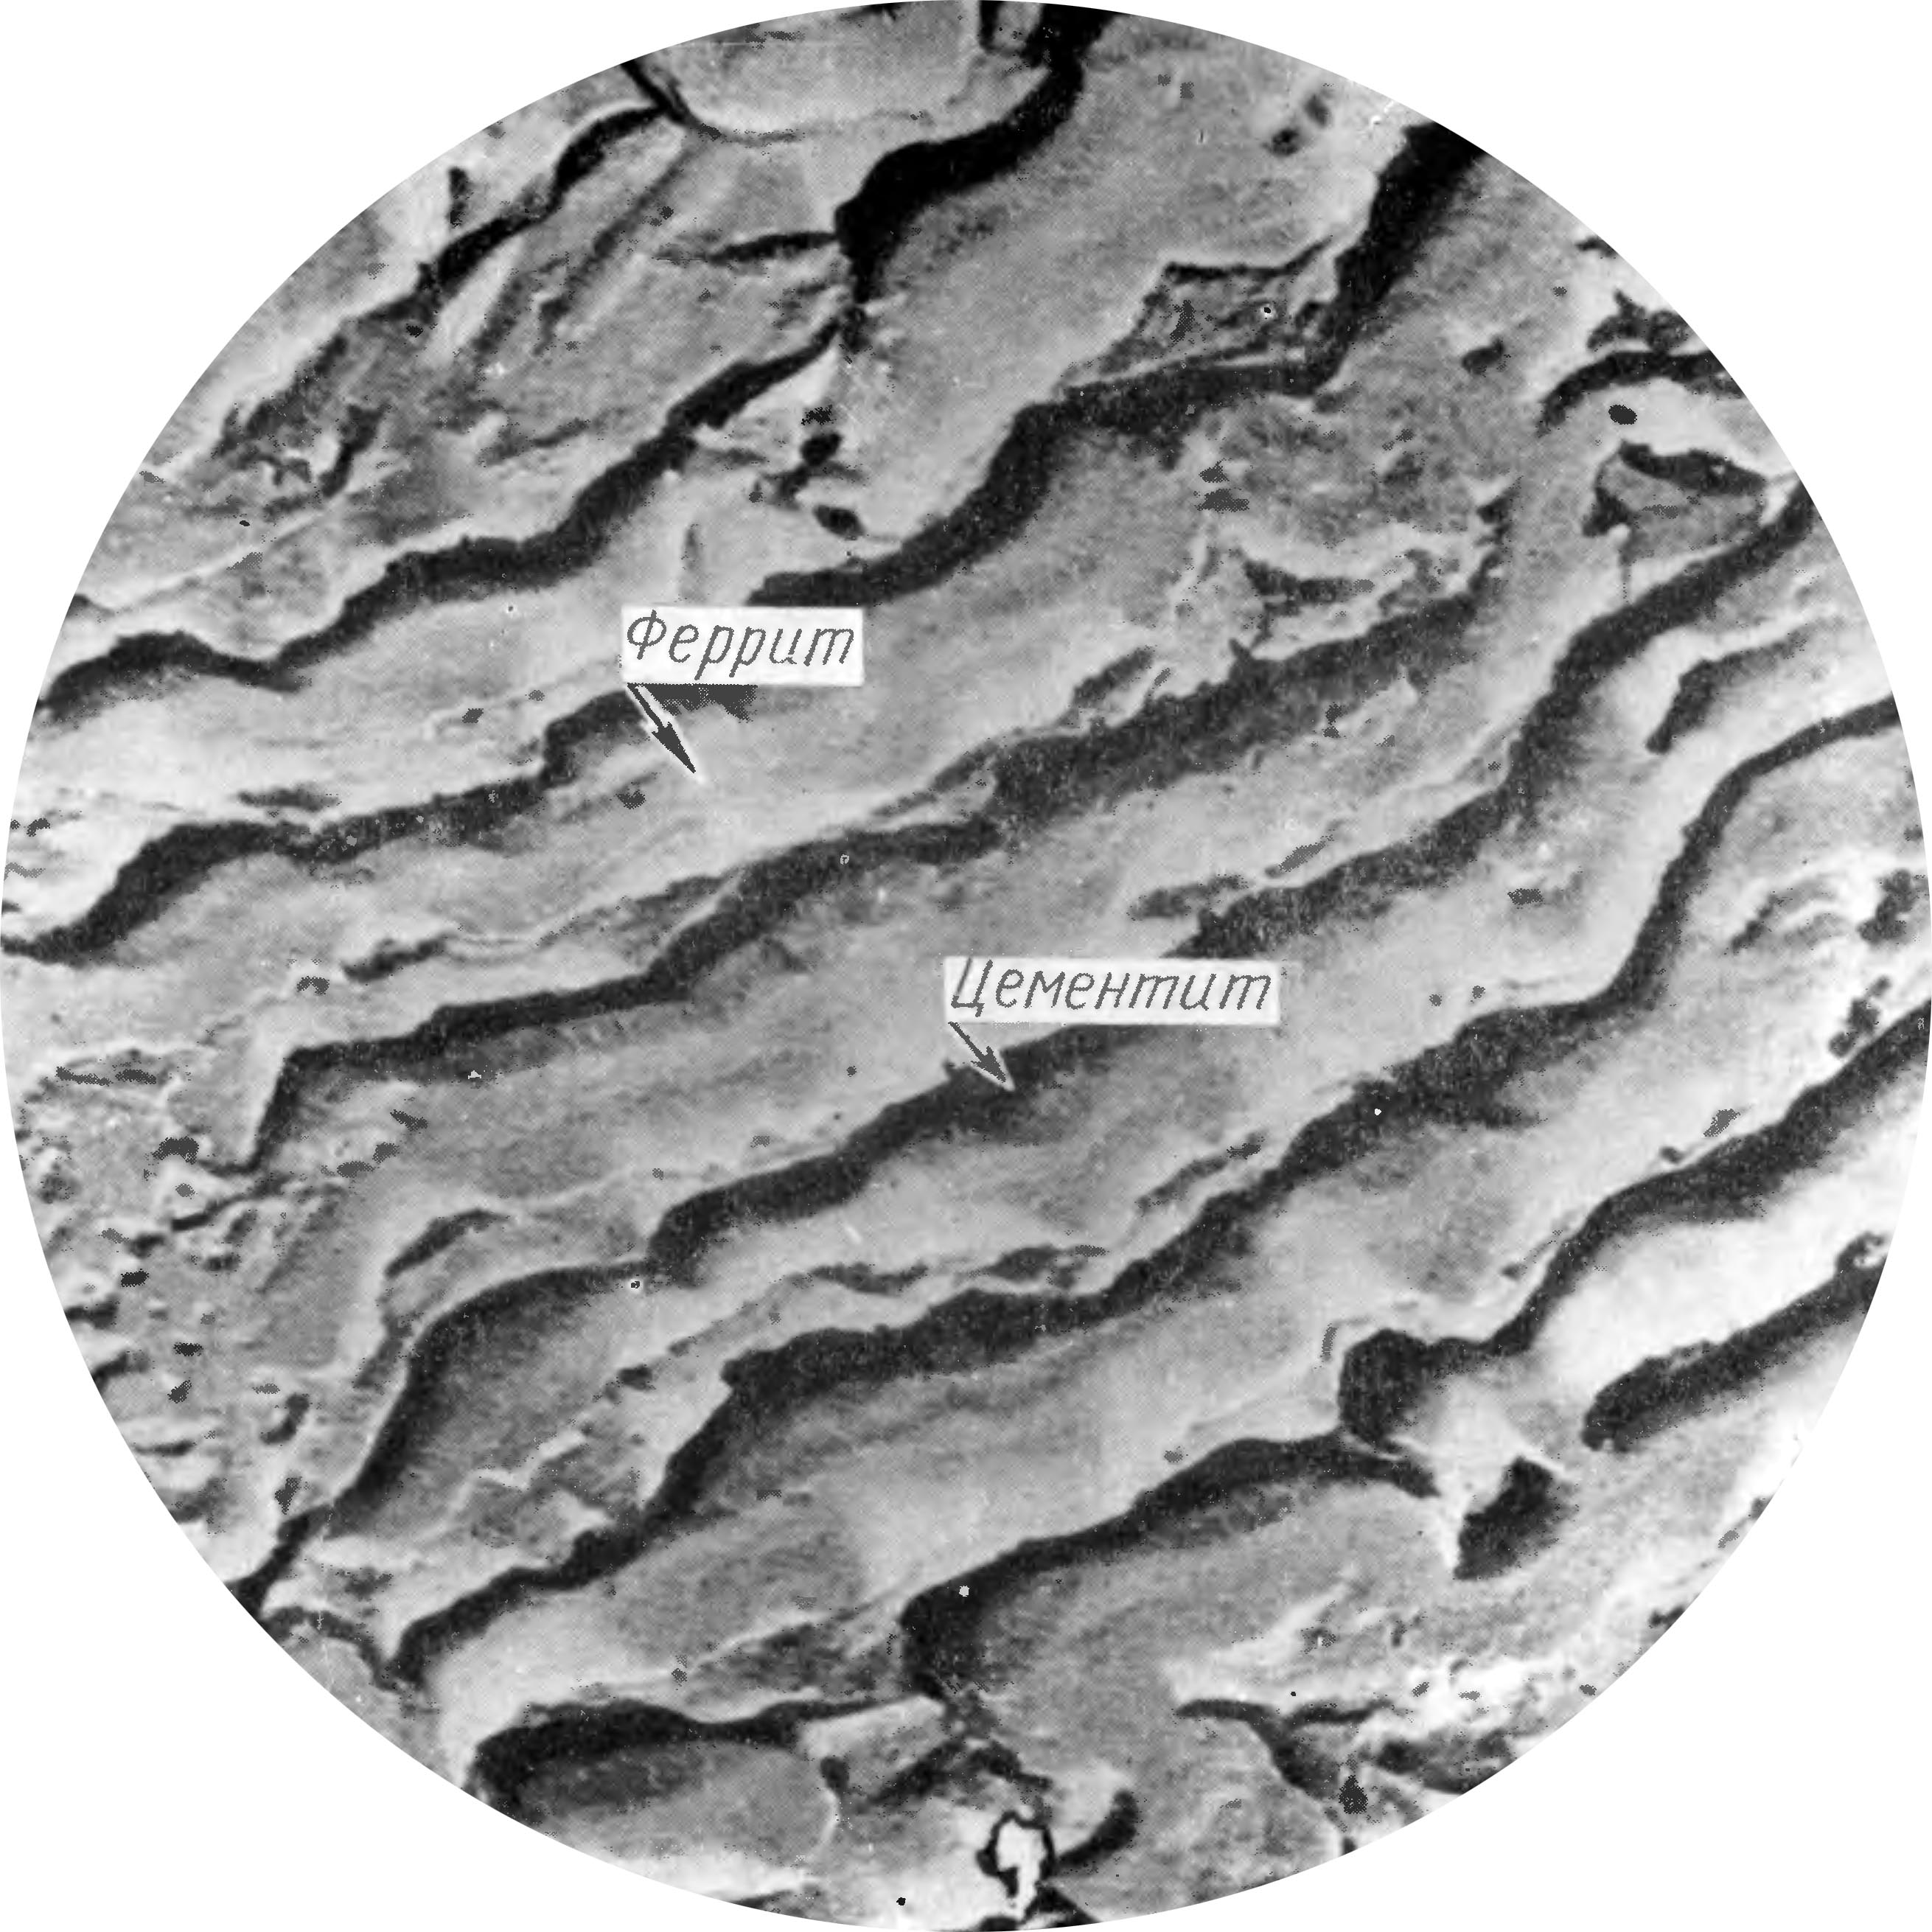
\includegraphics[scale=0.4]{images/пласт}
		\caption{ Перлит пластинчатый; х30000. Эвтектоид, состоящий из тонких пластинок цементита, наклоненных под углом к поверхности шлифа и расположенных на ферритной основе.}
	\end{figure}
	
	Однородный аустенит всегда превращается в пластинчатый перлит. Нагрев до высокой температуры, когда создаются условия для 
	образования более однородной структуры, способствует появлению пластинчатых структур. Неоднородный аустенит при всех степенях переохлаждения даёт зернистый перлит

	
	\newpage
	\section{Цели статьи}
	\begin{figure}[h!]
		\centering
%		\includegraphics[scale=0.5]{view}
		\caption{схема  на макетной плате}
	\end{figure}
	
	\section{Характеристики}
	\begin{itemize}
		\item f constant total carbide volume
		
		\item $f_u$ unspheroidized volume fraction
		
		\item degree of spheroidization E experimental\\
		\begin{equation}
				{f \over  f_u } = {1 \over 1-E }
				\label{eq:E_exp}
		\end{equation}
		
		\item degree of spheroidization E (Kostler)\\
		\begin{equation}
			E=m \times \lg t + b
			\label{eq:kostler}
		\end{equation}
	
		\item degree of spheroidization E (Atasoy)\\
		\begin{equation}
			E=1-A\times exp(-B\times r \times x^2 \times t)
			\label{eq:atasoy}
		\end{equation}
	
		\item spheroidization rate k (Atasoy)\\
		\begin{equation}
		B\times r \times x^2 \times t
			\label{eq:atasoyr}
		\end{equation}
		
		\item the mean particle size d (Dirnfeld)\\
		\begin{equation}
			d=a \times t^n
			\label{eq:dirnfeld}
		\end{equation}

		\item m, b, a, A, and B are constants to be determined from the
		available data
		
		\item the axis ratio of particle size r
		
		\item the mean thickness of non-spheroidized particles x
		
		\item annealing duration t 
		
		\item annealing temperature T
		
		\item The spheroidization rate $\nu_E$
		
		$\nu_E={dE \over{dt}}$
		
		\item hardness HV
		
		\item time–temperature parameter P
		
		$P=(C+\ln t) \times T$
		
		\item mean-intercept ferrite grain size L
		
		\item diameter of intra-grain carbides $d_{ig}$
		
		\item diameter of grain-boundary carbides $d_{gb}$
		
		\item volume fraction of second phase f
		
		\item mean surface-to-surface particle spacing $D_S$
		
			$D_S= ({2 \over {3f}})^{1 \over2} \times d \times (1-f))$
		
		
		\item ultimate tensile strength $R_m$
		
		\item reduction of area Z
		
		\item contribution from solid-solution strengthening $(\sigma_0)_{SS}$
		
		\item lower yield strength $R_{eL}$
		
		$R_{eL}=310D^{-1 \over 2}_S \times 460L^{-1 \over 2}$
		
		$R_{eL}=(\sigma_0)_{SS}+ 145D^{-1 \over 2}_S \times 460L^{-1 \over 2} $
		
		
		
		
	\end{itemize}
	\newpage
	
	\section{Эксперименты}
	
	
	За основу взята сталь AISI 1045 0.45C, 0.16Si, 0.69Mn, 0.05Cr, 0.023P, 0.019S.
	
	Взяли 9 образцои и провели отжиг каждой заготовки в течение 0, 0.5, 1, 2, 4, 8, 12, 16 и 24 часов
	соответственно при температура 680 $ \textdegree C$.
	
	\begin{figure}[h!]
		\centering
		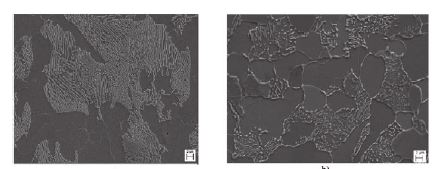
\includegraphics[scale=1.5]{images/0-0.5}
		\caption{ сфериодизация в течение 0 и 0,5 часов}
	\end{figure}
	
	\begin{figure}[h!]
		\centering
		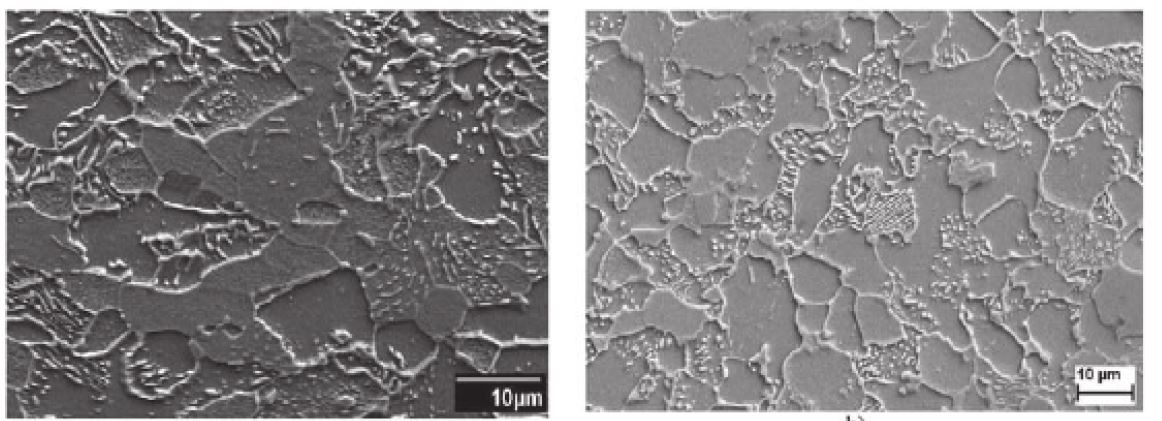
\includegraphics[scale=0.55]{images/12-16}
		\caption{ сфериодизация в течение 12 и 16 часов}
	\end{figure}
	
	После 8 часов отжига все еще остаются пластинчатые структуры, а после 12 - уже нет
	
	\begin{figure}[h!]
	\centering
	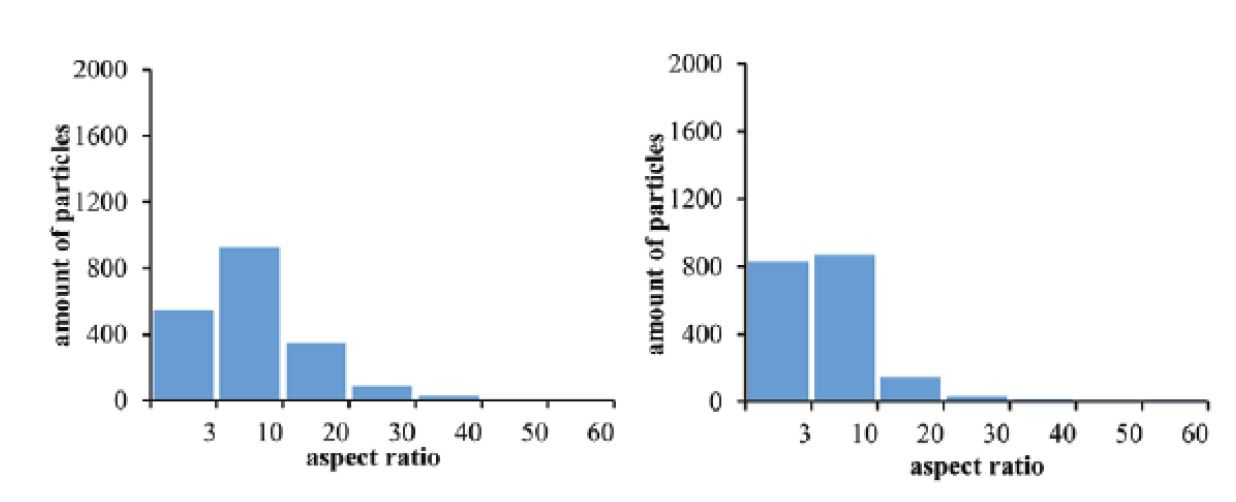
\includegraphics[scale=0.55]{images/ratio0-0.5}
	\caption{распределение количества частиц по соотношению сторон для структуры отжига 0 и 0,5 часов}
	\end{figure}
	
	\begin{figure}[h!]
		\centering
		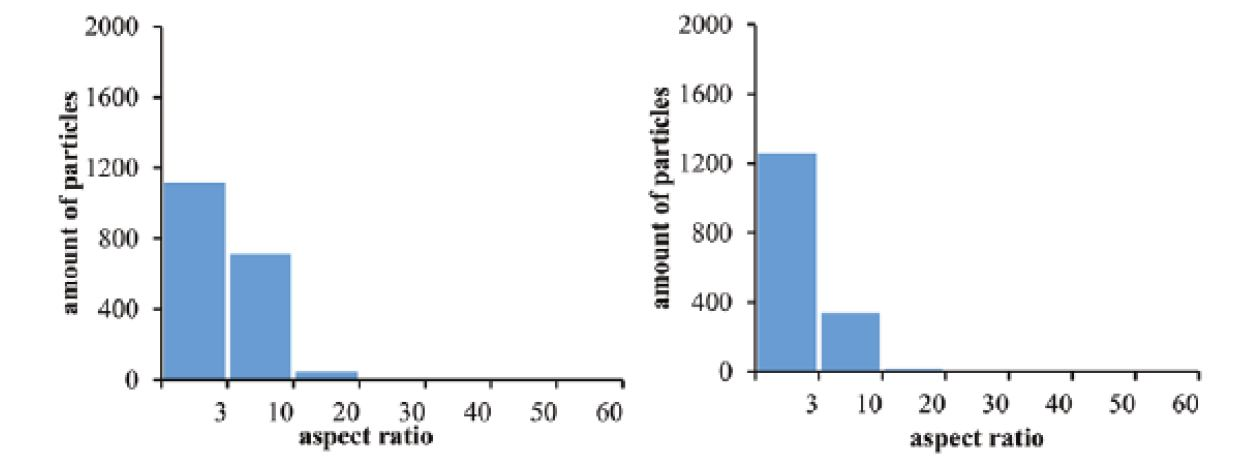
\includegraphics[scale=0.55]{images/ratio12-16}
		\caption{распределение количества частиц по соотношению сторон для структуры отжига 12 и 16 часов}
	\end{figure}

	\begin{figure}[h!]
	\centering
	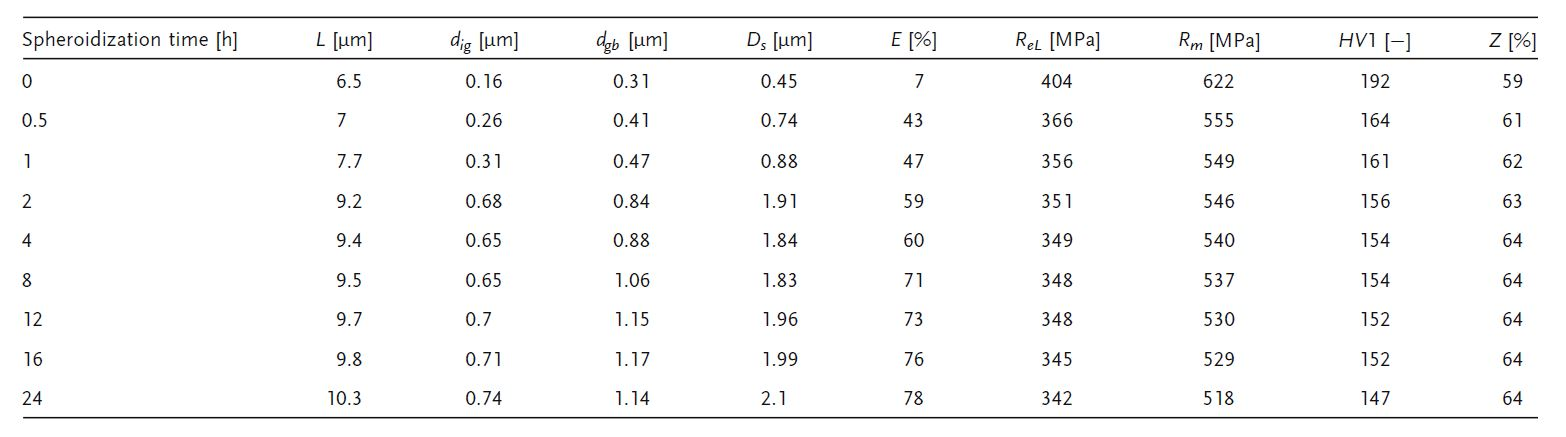
\includegraphics[scale=0.4]{images/table}
	\caption{измеренные механические характеристики металла}
	\end{figure}

	\newpage
	
	\FloatBarrier
	
	\section{Сравнение результатов экспериментов и  математических моделей}
	
		\begin{figure}[h!]
		\centering
		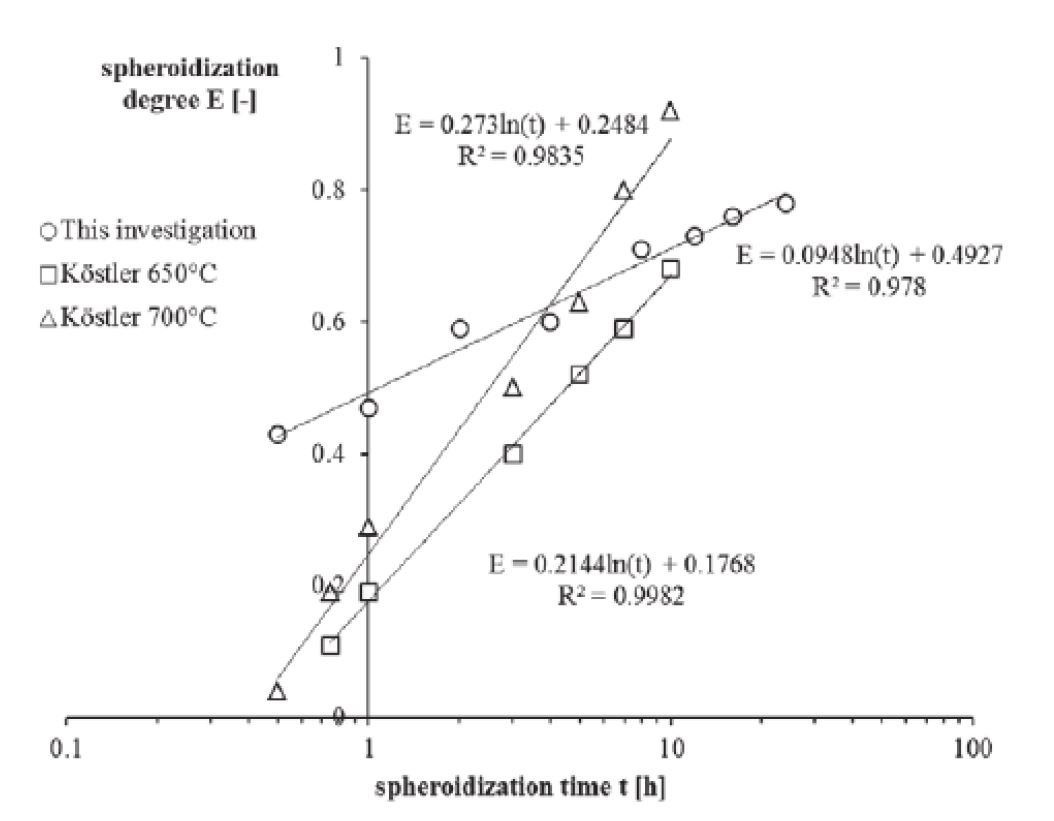
\includegraphics[scale=0.4]{images/kostler}
		\caption{сравнение модели Kostler (\ref{eq:kostler}) и экспериментальных данных (\ref{eq:E_exp}) для уровня сфериодизации от времени.}
	\end{figure}

	\begin{figure}[h!]
	\centering
	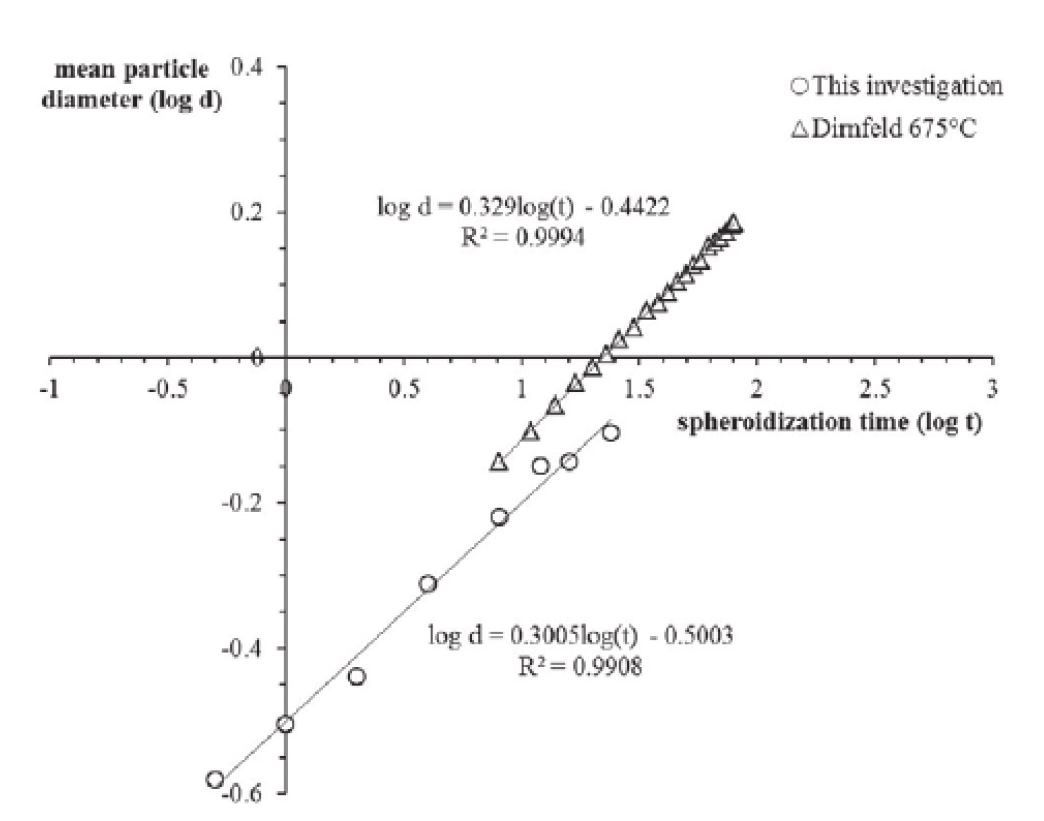
\includegraphics[scale=0.35]{images/dirnfeld}
	\caption{сравнение модели Dirnfeld (\ref{eq:dirnfeld}) и экспериментальных данных для среднего размера частиц цементита от времени}
	\end{figure}

	\begin{figure}[h!]
		\centering
		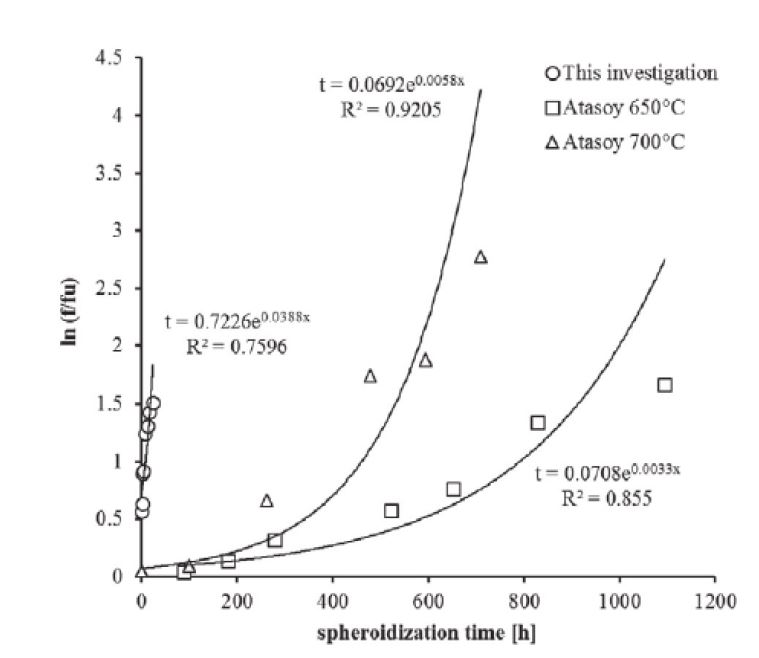
\includegraphics[scale=0.55]{images/fu}
		\caption{сравнение модели Atasoy (\ref{eq:atasoyr}) и экспериментальных данных отношения объема карбида к объему несфереодизированного карбида от времени. }
	\end{figure}
	
	\begin{figure}[h!]
		\centering
		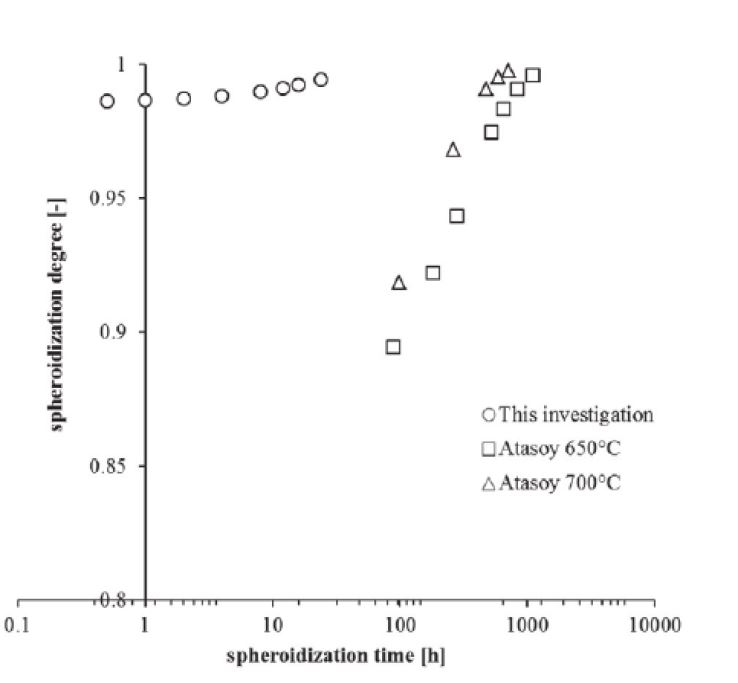
\includegraphics[scale=0.55]{images/degree}
			\caption{сравнение модели Atasoy (\ref{eq:atasoy}) и экспериментальных данных (\ref{eq:E_exp}) для уровня сфериодизации от времени}
	\end{figure}
	\newpage
	\section{Выводы}
	
	Механические характеристики сплава во многом зависят от процентного содержания примесей. В данной работе рассмотрен 
	характеристики сплава, которые зависят от содержания углерода и вида карбида железа. Проведенные исследования 
	полезны тем, что до этого не было статей, в которых подробно анализирутся и сравниваются полученные данные и математические модели для исследуемых величин.  
	
	\begin{itemize}
		\item проведение отжига в течение 24 часов не является гарантом того, что весь цементит перейдет из пластинчатой формы в сферическую
		
		\item не все модели (например модель Atasoy ) хорошо описывают характеристики сплавов
		
		\item результаты работы Dirnfeld дают хорошую точность для описания кинетический свойств сплава
		
		\item параметр Hollomon-Jaffe P дает наилучшие результаты для прогнозирования механичсеких характеристик 
		сплава
		
		\item очень сильное воздействие оказывается на частицы цементита, находящиеся в зерне, либо около его границы
	\end{itemize}
	
\end{document}